% arara: pdflatex: {interaction: nonstopmode, synctex: on,  shell: yes}
% arara: bibtex if found('log', 'Citation .* undefined')
% arara: pdflatex: {interaction: nonstopmode, synctex: on,  shell: yes}  if found('log', 'undefined references') or found('log', 'Rerun to') or found('log', 'Citation .* undefined')
% arara: pdflatex: {interaction: nonstopmode, synctex: on,  shell: yes}  if found('log', 'Rerun to') or found('log', 'Citation .* undefined')

\documentclass{cubeamer}
\input macros.tex
\input tikz.tex
\input acronyms.tex
\usetikzlibrary{positioning}
%%% Custom TikZ addons
\usetikzlibrary{crypto.symbols}
%\tikzset{shadows=no}  
\usetikzlibrary{decorations.pathreplacing}
\usetikzlibrary{arrows}
\usetikzlibrary{arrows.meta}
\usetikzlibrary{patterns}
\usetikzlibrary{shapes}
\usetikzlibrary{shadows}
\usetikzlibrary{calc}
\usetikzlibrary{math}

\hypersetup{
    colorlinks=true,
    linkcolor=blue,
    citecolor=green,
    urlcolor=cyan
}
\def\makethanks{%
    \begin{frame}
        \frametitle{\thankstitle}
        \thanksmessage
    \end{frame}
}
% in ``article'' mode there's no ``Thank you'' page
\mode<article>
{\providecommand\makethanks{}}


% commands for the title and message of the "Thank you" page
\def\thankstitle#1{\def\thankstitle{#1}}
\def\thanksmessage#1{\def\thanksmessage{#1}}
\thankstitle{}
\thanksmessage{{\huge {\color{red} Thank You} for your attention!} \\ \Large Any questions?}


\title[Block Cipher]{Tutorial on Block Ciphers}
% \subtitle{\green{National Workshop on Cryptology 2025, IIT Bhilai}}
\author[\red{Shibam}]{
    {\Large Shibam Ghosh}
}
% \date{January 29, 2026} % or whatever the date you are presenting in is
\institute[IIT Hyderabad]{\textcolor{redd}{{\Large Department of CSE, IIT Hyderabad}}}
% \institute[INRIA, Paris]{INRIA, Paris, France}
\date{\today} % or whatever the date you are presenting in is

 \AtBeginSection[] { %
    \begin{frame}[noframenumbering]
        \frametitle{Plan of this Section}
        \tableofcontents[
        currentsection,
        currentsubsection,
        sectionstyle=show/shaded,
        subsectionstyle=show/show/hide,
        subsubsectionstyle=hide]
    \end{frame}
}

\tcbuselibrary{many}
% \usepackage[many]{tcolorbox}
\setbeamertemplate{itemize item}{$\blacktriangleright$}
\setbeamertemplate{itemize subitem}{$\triangleright$}
\setbeamertemplate{itemize subsubitem}{$\rhd$}

% Later, reload hyperref with your desired options:
\hypersetup{
    colorlinks=true,
    linkcolor=blue,
    citecolor=green,
    urlcolor=cyan
}

% -------------------------------------------------------
% Define Cyan Color for Title
% -------------------------------------------------------
\definecolor{myctyan}{RGB}{0,180,200}
\definecolor{mytheme}{RGB}{0, 51, 102}
\definecolor{cardbg}{RGB}{235, 242, 252}  % Light blue tint
% -------------------------------------------------------
% Override Frame Title Template
% -------------------------------------------------------
\setbeamertemplate{frametitle}{
    \vspace{0.1cm}
    \textcolor{mytheme}{\Large\textbf{\insertframetitle}}
    \vspace{0.05cm}
}

% -------------------------------------------------------
% Remove Navigation Symbols
% -------------------------------------------------------
\setbeamertemplate{navigation symbols}{}

% -------------------------------------------------------
% Optional: Clean Footline
% -------------------------------------------------------
\setbeamertemplate{footline}{
    \begin{beamercolorbox}[wd=\paperwidth,ht=0.2cm,dp=0.2cm]{footline}
        \hspace{0.2cm}
        
\includegraphics[scale=0.03]{img/iith.png}
        \hfill
        \textcolor{gray}{\tiny\insertframenumber\,/\,\inserttotalframenumber}
        \hspace{0.5cm}
    \end{beamercolorbox}
}

% ---- ADD THIS AT THE END OF YOUR PREAMBLE ----
\makeatletter
\beamer@frametopskip=0pt plus 0pt\relax       % No flexible space on top
\beamer@framebottomskip=0pt plus 1fill\relax  % All flexible space goes to bottom
\makeatother


\usepackage{etoolbox}
\makeatletter
% Remove top filler from frame body
\patchcmd{\beamer@calculateheadfoot}{\vfill}{}{}{}
\makeatother
% ----------------------------------------------

% Put this in your preamble

% Section slide
\AtBeginSection[]{
    \begin{frame}[plain, noframenumbering]
        \begin{center}
            \vfill
            \textcolor{myctyan}{\rule{0.6\textwidth}{1.5pt}}
            \vspace{0.3cm}

            \textcolor{myctyan}{\Huge\textbf{\insertsectionhead}}

            \vspace{0.3cm}
            \textcolor{myctyan}{\rule{0.6\textwidth}{1.5pt}}
            \vfill
        \end{center}
    \end{frame}
}

% Subsection slide
\AtBeginSubsection[]{
    \begin{frame}[plain, noframenumbering]
        \begin{center}
            \vfill

            % Show parent section in smaller text above
            \textcolor{myctyan!60}{\large\textbf{\insertsectionhead}}

            \vspace{0.3cm}
            \textcolor{myctyan}{\rule{0.4\textwidth}{0.8pt}}
            \vspace{0.3cm}

            % Show subsection in larger text below
            \textcolor{myctyan}{\LARGE\textbf{\insertsubsectionhead}}

            \vfill
        \end{center}
    \end{frame}
}


\begin{document}

\maketitle

\begin{frame}[t]
    \frametitle{Table of contents}
    \tableofcontents
\end{frame}
%\cutoc

\section{Introduction}

\begin{frame}
\frametitle{Symmetric-Key Cryptography}
    \centering
    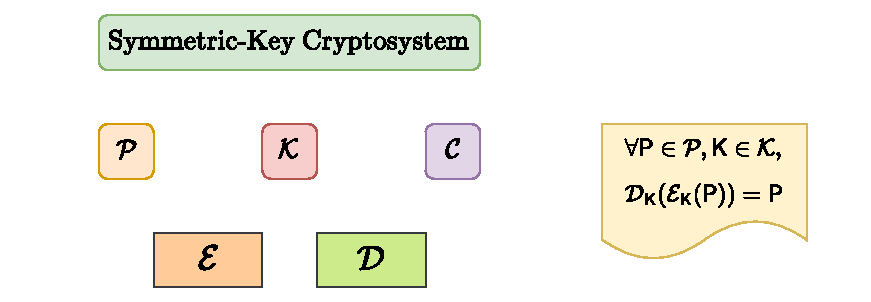
\includegraphics[width=12cm]{./fig/symm.pdf}
    \vfill

    \pause
    \centering
    e.g., Block ciphers, stream ciphers, hash functions, MACs, \ldots
\end{frame}

\begin{frame}
    \frametitle{Block Cipher}
    \centering
    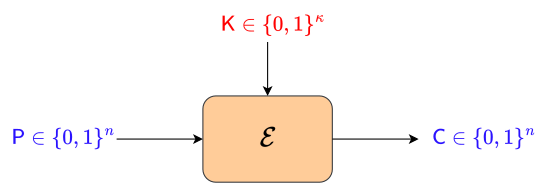
\includegraphics[width=10cm]{./fig/bc.png}
    \vfill
    \pause

    \begin{itemize}
        \item $\mathcal{E}: \{0,1\}^n \times \{0,1\}^{\kappa} \to \{0,1\}^n \text{ s.t. } \cc = \mathcal{E}(\pp, \kk)$
        \item $\mathcal{E}_{\kk}: \{0,1\}^n \to \{0,1\}^n \text{ s.t. } \cc = \mathcal{E}_{\kk}(\pp)$
    \end{itemize}
\end{frame}

\tikzset{
    blockcipher1/.style={
		fill=blue!10,
		rectangle,
		draw=bluee,
		semithick,
		inner sep=0pt,
		minimum height=1cm,
		minimum width=1cm,
		rounded corners=1mm,
	},
    blockcipher2/.style={
		fill=teal!10,
		rectangle,
		draw=green,
		semithick,
		inner sep=0pt,
		minimum height=1cm,
		minimum width=1cm,
		rounded corners=1mm,
	},
    roundfunction/.style={
		fill=blue!10,
		rectangle,
		draw=violet,
		semithick,
		inner sep=0pt,
		minimum height=1cm,
		minimum width=1cm,
		rounded corners=1mm,
	},
}


\begin{frame}
\frametitle{Iterated Block Cipher}
\begin{figure}
	\centering
	{%
		% \setlength{\fboxsep}{0.5pt}%
		% \setlength{\fboxrule}{0.5pt}%
		% \fbox{
            \resizebox{\textwidth}{!}{
				\begin{tikzpicture}[scale=1]

				\tikzstyle{every node}=[transform shape];
				\tikzstyle{every node}=[node distance=1.5cm];

                \draw[semithick, color = bluee, rounded corners=1mm] (-0.9,-0.6) rectangle (7.3,2.8) node[above left] {Block Cipher};

				% Expansion Algorithm
				\node (KS) [draw,trapezium,trapezium left angle=40,trapezium right angle=40,minimum height=0.75cm,semithick,fill=blue!15,shift={(3.2,2)},inner xsep=40pt] {Key Schedule};

                \node (k) [above=0.8cm of KS] {$\kk$};
				\path[line] (k) edge (KS);

				% Data path
                \node[roundfunction] (R-1) {$R_1$};
                \node [left of=R-1] (p) {$\pp$};
				\path[line] (p) edge (R-1);

				\node[roundfunction, right of=R-1] (R-2) {$R_2$};
				\path[line] (R-1) edge node[below] {} (R-2);


				\node (dots)[right of=R-2] {$\cdots\cdots$};
				\path[line] (R-2) edge (dots);
				\node[roundfunction, right of=dots] (R-3){$R_{r-1}$};
				\path[line] (dots) edge (R-3) ;


				\node[roundfunction, right of=R-3] (R-4)[node distance=1.9cm] {$R_r$};
				\path[line] (R-3) edge node[below] {} (R-4);
                \node [right of=R-4,node distance=1.5cm] (c) {$\cc$};
				\path[line] (R-4) edge (c);

				%% Subkeys
				\node (k-0) [above=1.15cm of R-1] {};
				\path[line] (k-0) edge node[right] {\small $k_{1}$} (R-1);

				\node (k-1) [above=1.15cm of R-2] {};
				\path[line] (k-1) edge node[right] {\small $k_{2}$} (R-2);

				\node (k-2) [above=1.15cm of R-3] {};
				\path[line] (k-2) edge node[right] {\small $k_{r-1}$} (R-3);

				\node (k-3) [above=1.15cm of R-4] {};
				\path[line] (k-3) edge node[right] {\small $k_{r}$} (R-4);

				\end{tikzpicture}

			}
		}%
	% }%
	% \caption{\label{fig:product}Iterated block cipher.}
\end{figure}
\end{frame}
\begin{frame}
\frametitle{Iterated Tweakable Block Cipher with TWEAKEY Schedule}
\begin{figure}
	\centering
	{%
		% \setlength{\fboxsep}{0.5pt}%
		% \setlength{\fboxrule}{0.5pt}%
		% \fbox{
            \resizebox{\textwidth}{!}{
				\begin{tikzpicture}[scale=1]

				\tikzstyle{every node}=[transform shape];
				\tikzstyle{every node}=[node distance=1.5cm];

                \draw[semithick, color = bluee, rounded corners=1mm] (-0.9,-0.6) rectangle (7.3,2.8) node[above left] {TBC};

				% Expansion Algorithm
                \node (KS) [draw,trapezium,trapezium left angle=40,trapezium right angle=40,minimum height=0.55cm,semithick,fill=blue!15,shift={(3.2,2)},inner xsep=40pt] {{\small \red{TWEA}KEY Schedule}};

                \node (k) [above=0.8cm of KS] {$\kk, T$};
				\path[line] (k) edge (KS);

				% Data path
                \node[roundfunction] (R-1) {$R_1$};
                \node [left of=R-1] (p) {$\pp$};
				\path[line] (p) edge (R-1);

				\node[roundfunction, right of=R-1] (R-2) {$R_2$};
				\path[line] (R-1) edge node[below] {} (R-2);


				\node (dots)[right of=R-2] {$\cdots\cdots$};
				\path[line] (R-2) edge (dots);
				\node[roundfunction, right of=dots] (R-3){$R_{r-1}$};
				\path[line] (dots) edge (R-3) ;


				\node[roundfunction, right of=R-3] (R-4)[node distance=1.9cm] {$R_r$};
				\path[line] (R-3) edge node[below] {} (R-4);
                \node [right of=R-4,node distance=1.5cm] (c) {$\cc$};
				\path[line] (R-4) edge (c);

				%% Subkeys
				\node (k-0) [above=1.15cm of R-1] {};
				\path[line] (k-0) edge node[right] {\small $tk_{1}$} (R-1);

				\node (k-1) [above=1.15cm of R-2] {};
				\path[line] (k-1) edge node[right] {\small $tk_{2}$} (R-2);

				\node (k-2) [above=1.15cm of R-3] {};
				\path[line] (k-2) edge node[right] {\small $tk_{r-1}$} (R-3);

				\node (k-3) [above=1.15cm of R-4] {};
				\path[line] (k-3) edge node[right] {\small $tk_{r}$} (R-4);

				\end{tikzpicture}

			}
		}%
	% }%
\end{figure}
% \pause
% {\tiny \red{Chilow and chichi: New constructions for code encryption. EUROCRYPT}, volume 15601 of Lecture Notes in Computer Science, pages 212–243. Springer, 2025}
\end{frame}

\section{The Advanced Encryption Standard (AES)}
% --- SLIDE 1 ---
\begin{frame}{The Advanced Encryption Standard}
    \begin{itemize}
    \item \textbf{The Competition of (1997)} by NIST (National Institute of Standards and Technology) for a highly secure, efficient, and royalty-free cipher
   \pause
   \item \textbf{The Finalists (1999):} Out of 15 initial submissions, 5 finalists were selected: MARS, RC6, \textbf{Rijndael}, Serpent, and Twofish.
   \pause
   \item \textbf{The Winner (2000):} \textbf{Rijndael}, designed by Belgian cryptographers Joan Daemen and Vincent Rijmen
       \begin{itemize} 
           \item Excellent balance of security and performance 
           \item Flexibility across hardware and software
       \end{itemize}
   \pause
   \item \textbf{Standardization (2001):} Officially published as FIPS PUB 197
    \end{itemize}
\end{frame}

% --- SLIDE 2 ---
\begin{frame}{Round Function of \tx{AES}}
    \begin{itemize}
        \item \tx{AES} has an SP (\red{substitution}-\green{permutation}) network structure.
        \pause
    \item Block size: $n = 128$ bits, i.e., $\pp \in \{0,1\}^{128} \text{ or } \pp \in \mathbb{F}_2^{128} \text{ or } \pp \in (\mathbb{F}_{2^{8}})^{16}$
        \item Key size: $\kappa =  128, 192, \text{ or } 256$
     \end{itemize}
    
     \pause
    \begin{center}
    \begin{tikzpicture}[scale=0.8, every node/.style={scale=0.8}]
        \def\gs{0.6} % grid cell size

        % Grid 1: Full State
        \begin{scope}[xshift=0cm]
            \draw[step=\gs] (0,0) grid (4*\gs, 4*\gs);
            \foreach \x in {0,...,3} {
                \foreach \y in {0,...,3} {
                    \node at (\x*\gs+\gs/2, 4*\gs-\y*\gs-\gs/2) {\large $\pgfmathparse{int(\x*4+\y)}\pgfmathresult$};
                }
            }
        \end{scope}

        % Grid 2: SubBytes
        \begin{scope}[xshift=4.2cm]
            \draw[step=\gs] (0,0) grid (4*\gs, 4*\gs);
            % Highlight cell (0, 3) relative to reading order -> top right
            \node[draw, circle, thick, minimum size=0.55cm] at (3*\gs+\gs/2, 4*\gs-\gs/2) {};
            % Bottom row elements
            \node at (0*\gs+\gs/2, \gs/2) {\large 3};
            \node at (1*\gs+\gs/2, \gs/2) {\large 7};
            \node at (2*\gs+\gs/2, \gs/2) {\large 11};
            \node at (3*\gs+\gs/2, \gs/2) {\large 15};
            % Highlight bottom row
            \draw[thick] (2*\gs, \gs/2) ellipse (2*\gs cm and 0.28cm);
        \end{scope}

        % Grid 3: ShiftRows
        \begin{scope}[xshift=8.4cm]
            \draw[step=\gs] (0,0) grid (4*\gs, 4*\gs);
            % Bottom row elements shifted
            \node at (0*\gs+\gs/2, \gs/2) {\large 15};
            \node at (1*\gs+\gs/2, \gs/2) {\large 3};
            \node at (2*\gs+\gs/2, \gs/2) {\large 7};
            \node at (3*\gs+\gs/2, \gs/2) {\large 11};
            % Highlight bottom row
            \draw[thick] (2*\gs, \gs/2) ellipse (2*\gs cm and 0.28cm);
            % Highlight third column
            \draw[pattern=north east lines, thick] (2*\gs+\gs/2, 2*\gs) ellipse (0.28cm and 2*\gs cm);
        \end{scope}

        % Grid 4: MixColumns
        \begin{scope}[xshift=12.6cm]
            \draw[step=\gs] (0,0) grid (4*\gs, 4*\gs);
            % Highlight third column
            \draw[pattern=north east lines, thick] (2*\gs+\gs/2, 2*\gs) ellipse (0.28cm and 2*\gs cm);
        \end{scope}

        % Straight Arrows between grids
        \draw[->, thick, >=stealth] (4*\gs, 2*\gs) -- node[above] {\Large SB} (4.2, 2*\gs);
        \draw[->, thick, >=stealth] (4.2+4*\gs, 2*\gs) -- node[above] {\Large SR} (8.4, 2*\gs);
        \draw[->, thick, >=stealth] (8.4+4*\gs, 2*\gs) -- node[above] {\Large MC} (12.6, 2*\gs);

        % Curved Arrows showing specific operations
        \draw[->, thick, >=stealth] (1.5*\gs, 4*\gs) to[out=60, in=120] node[above] {\Large SubBytes} (4.2+3*\gs+\gs/2, 4*\gs);
        \draw[->, thick, >=stealth] (4.2+2*\gs, -0.1) to[out=-60, in=-120] node[below] {\Large ShiftRows} (8.4+2*\gs, -0.1);
        \draw[->, thick, >=stealth] (8.4+2*\gs+\gs/2, -0.1) to[out=-60, in=-120] node[below] {\Large MixColumns} (12.6+2*\gs+\gs/2, -0.1);

        % AddRoundKey at the end
        \draw[->, thick, >=stealth] (12.6+4*\gs, 2*\gs) -- (16, 2*\gs);
        \node[draw, circle, inner sep=0pt, thick, minimum size=15pt, fill=white] (ark) at (15.5, 2*\gs) {\Large $\oplus$};
        \draw[->, thick, >=stealth] (15.5, 2*\gs-1.5) -- node[right] {\Large $K_i$} (ark);
        \node at (15.5, 2*\gs+0.8) {\Large ARK};

    \end{tikzpicture}
    \end{center}
\end{frame}

\begin{frame}
\frametitle{Round Function of \tx{AES} (cont.)}
    \centering
    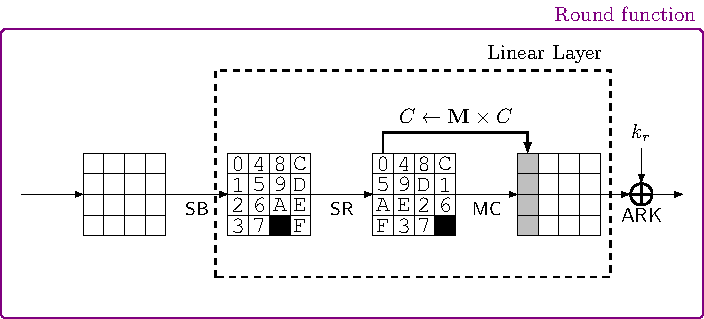
\includegraphics[width=12cm]{./fig/spn_matrix.pdf}
    
    \pause
    
    \centering
    Number of rounds depends on the key length (10/12/14, respectively).
\end{frame}


% --- SLIDE 3 & 4 ---
\begin{frame}{The MixColumns Operation}
    \begin{itemize}
        \item MixColumns treats each column of four bytes as four elements over $GF(2^8)$:
        \vspace{0.5em}
        \[
        \begin{bmatrix}
        s'_0 \\
        s'_1 \\
        s'_2 \\
        s'_3
        \end{bmatrix}
        =
        \begin{bmatrix}
        2 & 3 & 1 & 1 \\
        1 & 2 & 3 & 1 \\
        1 & 1 & 2 & 3 \\
        3 & 1 & 1 & 2
        \end{bmatrix}
        \begin{bmatrix}
        s_0 \\
        s_1 \\
        s_2 \\
        s_3
        \end{bmatrix}
        \]
        \vspace{0.5em}

        \uncover<2->{
        \item The irreducible polynomial of $GF(2^8)$ is $x^8 + x^4 + x^3 + x + 1$
        }
    \end{itemize}
\end{frame}

% --- SLIDE 1: Representation ---
\begin{frame}{``Galois Field with $2^8$ elements'': Representation}
    \begin{itemize}
        \item A state of \tx{AES} is a sequence of bytes or elements of finite field $GF(2^8)$ or $\mathbb{F}_{2^{8}}$.
        \pause
        \item A byte consists of 8 bits, i.e., binary string of length 8.
         \pause
        \item Each element of $GF(2^8)$ which can be represented as a polynomial of degree up to 7 with coefficients are only 0 and 1
    \end{itemize}
    \vspace{0.5em}
    \begin{center}
        \renewcommand{\arraystretch}{1.2}
        \begin{tabular}{c c l}
            \toprule
            \textbf{Integer} & \textbf{Binary} & \textbf{Polynomial in $GF(2^8)$} \\
            \midrule
            0  & 00000000 & $0$ \\
            1  & 00000001 & $1$ \\
            2  & 00000010 & $x$ \\
            3  & 00000011 & $x + 1$ \\
            16 & 00010000 & $x^4$ \\
            21 & 00010101 & $x^4 + x^2 + 1$ \\
            \bottomrule
        \end{tabular}
    \end{center}
\end{frame}

% --- SLIDE 2: Addition ---
\begin{frame}{Addition in $GF(2^8)$}
    \begin{itemize}
        \item Addition in a finite field works by adding the underlying polynomials
        \item No carry bits are generated as coefficients are modulo 2, $1 + 1 = 0$
        \item Therefore, addition, subtraction, and \textbf{XOR ($\oplus$)} are the exact same operation! 
    \end{itemize}
    \pause

    % Side-by-side examples
    \begin{columns}[T] % [T] aligns the tops of the columns
        \begin{column}{0.48\textwidth}
            \begin{block}{Example 1: addition}
                \begin{align*}
                    1 + 2 &\equiv (1) + (x) \\
                          &= x + 1 \\
                          &\equiv 00000011_2 \\
                          &= \mathbf{3}
                \end{align*}
            \end{block}
        \end{column}

        \begin{column}{0.48\textwidth}
            \uncover<2->{
            \begin{block}{Example 2: Binary wraparound}
                \begin{align*}
                    2 + 2 &\equiv (x) + (x) \\
                          &= 2x \\
                          &\equiv 0x \quad \text{\footnotesize (Since } 2 \bmod 2 = 0\text{)} \\
                          &= \mathbf{0}
                \end{align*}
            \end{block}
            }
        \end{column}
    \end{columns}
\end{frame}

% --- SLIDE 3: Multiplication ---
\begin{frame}{Multiplication in $GF(2^8)$}
    \begin{itemize}
        \item Multiplication works just like standard polynomial multiplication.
        \item \textbf{Catch:} If the resulting degree is $\ge 8$, it falls outside $GF(2^8)$.
        \item \textbf{Fix:} Replace $x^8$ using the \textit{irreducible polynomial}: $\mathbf{x^4 + x^3 + x + 1}$.
    \end{itemize}

    \begin{block}{Examples}
        \begin{itemize}
            \item $2 \times 2 \equiv (x) \times (x) = x^2 \equiv 00000100_2 = \mathbf{4}$
            \pause
            \item What is $16 \times 16$? \pause $16 \times 16 \equiv (x^4) \times (x^4) = \mathbf{x^8}$
        \end{itemize}
        \pause
        \begin{align*}
            x^8 &\equiv x^8 \oplus (x^8 + x^4 + x^3 + x + 1) = x^4 + x^3 + x + 1 \\
                &\equiv 00011011_2 = \mathbf{27}
        \end{align*}
    \end{block}
\end{frame}

% --- SLIDE 4: Multiplication by 2 and 3 ---
\begin{frame}{Multiplication by 2 and 3 in $GF(2^8)$}
    \begin{itemize}
        \item \textbf{Multiply by 2 (Polynomial $x$):}
        \begin{itemize}
            \item \textbf{Left Shift:} Left shift the binary string by one position
            \item \textbf{Reduce:} If the leftmost bit (MSB) is 1, XOR the result with the reducing polynomial ($00011011_2$).
        \end{itemize}
        \item \textbf{Multiply by 3 (Polynomial $x+1$):}
        \begin{itemize}
            \item \textbf{Action:} Multiply by 2 (shift \& reduce), then XOR with the original value.
        \end{itemize}
    \end{itemize}
    \pause
    \begin{columns}[T]
        \begin{column}{0.48\textwidth}
            \begin{block}{Example: $27 \times 2$}
                $27$ in binary: $\mathbf{00011011_2}$ \\
                \vspace{0.5em}
                \textbf{1. Left shift by 1:}\\
                $00011011_2 \ll 1 = 00110110_2$ \\
                \textbf{2. Reduce?} No \\
                \textbf{Result:} $00110110_2 = \mathbf{54}$
            \end{block}
        \end{column}

        \begin{column}{0.48\textwidth}
            \uncover<2->{
            \begin{block}{Example: $27 \times 3$}
                Formula: $(27 \times 2) \oplus 27$ \\
                From the previous step: \\
                $27 \times 2 = 00110110_2$ \\
                \textbf{XOR with original value (27):} \\
                \vspace{0.2em}
                \begin{tabular}{@{}r@{\;}l@{\;}l}
                           & $00110110_2$ & ($54$) \\
                  $\oplus$ & $00011011_2$ & ($27$) \\
                  \hline
                           & $\mathbf{00101101_2}$ & ($\mathbf{45}$)
                \end{tabular}
            \end{block}
            }
        \end{column}
    \end{columns}
\end{frame}

% --- SLIDE 5: Multiplication by 2 as a Matrix ---
\begin{frame}{Multiplication by 2 as a Matrix Operation}
    \begin{itemize}
        \item Let the byte be a column vector $\mathbf{b} = [b_0, b_1, b_2, b_3, b_4, b_5, b_6, b_7]^T$, where $b_0$ is the LSB ($x^0$) and $b_7$ is the MSB ($x^7$).
    \end{itemize}
    
    \[
    \begin{bmatrix}
    b'_0 \\ b'_1 \\ b'_2 \\ b'_3 \\ b'_4 \\ b'_5 \\ b'_6 \\ b'_7
    \end{bmatrix}
    =
    \left[
    \begin{array}{ccccccc|c}
    0 & 0 & 0 & 0 & 0 & 0 & 0 & \mathbf{1} \\
    \red{1} & 0 & 0 & 0 & 0 & 0 & 0 & \mathbf{1} \\
    0 & \red{1} & 0 & 0 & 0 & 0 & 0 & \mathbf{0} \\
    0 & 0 & \red{1} & 0 & 0 & 0 & 0 & \mathbf{1} \\
    0 & 0 & 0 & \red{1} & 0 & 0 & 0 & \mathbf{1} \\
    0 & 0 & 0 & 0 & \red{1} & 0 & 0 & \mathbf{0} \\
    0 & 0 & 0 & 0 & 0 & \red{1} & 0 & \mathbf{0} \\
    0 & 0 & 0 & 0 & 0 & 0 & \red{1} & \mathbf{0}
    \end{array}
    \right]
    \begin{bmatrix}
    b_0 \\ b_1 \\ b_2 \\ b_3 \\ b_4 \\ b_5 \\ b_6 \\ b_7
    \end{bmatrix}
    \]
    \begin{itemize}
        \item \textbf{Sub-diagonal of 1s:} Performs the standard left shift ($b'_i = b_{i-1}$).
        \item \textbf{Rightmost Column:} Adds the reduction polynomial only when the MSB ($b_7$) is $1$.
    \end{itemize}
\end{frame}

% --- SLIDE 5 ---
\begin{frame}{The SubBytes Operation}
    \begin{itemize}
        \item Given input $x$, compute $y = x^{-1}$ (over the same field, with $0 \triangleq 0^{-1}$).
        \item Then compute the output as:
        \[
        \setlength{\arraycolsep}{4pt} % Slightly compress matrix width
        \begin{bmatrix}
        z_0 \\ z_1 \\ z_2 \\ z_3 \\ z_4 \\ z_5 \\ z_6 \\ z_7
        \end{bmatrix}
        =
        \begin{bmatrix}
        1 & 0 & 0 & 0 & 1 & 1 & 1 & 1 \\
        1 & 1 & 0 & 0 & 0 & 1 & 1 & 1 \\
        1 & 1 & 1 & 0 & 0 & 0 & 1 & 1 \\
        1 & 1 & 1 & 1 & 0 & 0 & 0 & 1 \\
        1 & 1 & 1 & 1 & 1 & 0 & 0 & 0 \\
        0 & 1 & 1 & 1 & 1 & 1 & 0 & 0 \\
        0 & 0 & 1 & 1 & 1 & 1 & 1 & 0 \\
        0 & 0 & 0 & 1 & 1 & 1 & 1 & 1
        \end{bmatrix}
        \begin{bmatrix}
        y_0 \\ y_1 \\ y_2 \\ y_3 \\ y_4 \\ y_5 \\ y_6 \\ y_7
        \end{bmatrix}
        \oplus
        \begin{bmatrix}
        1 \\ 1 \\ 0 \\ 0 \\ 0 \\ 1 \\ 1 \\ 0
        \end{bmatrix}
        \]
    \end{itemize}
\end{frame}

\begin{frame}{\tx{AES} SubBytes Operation as a Table Lookup}
    \centering
    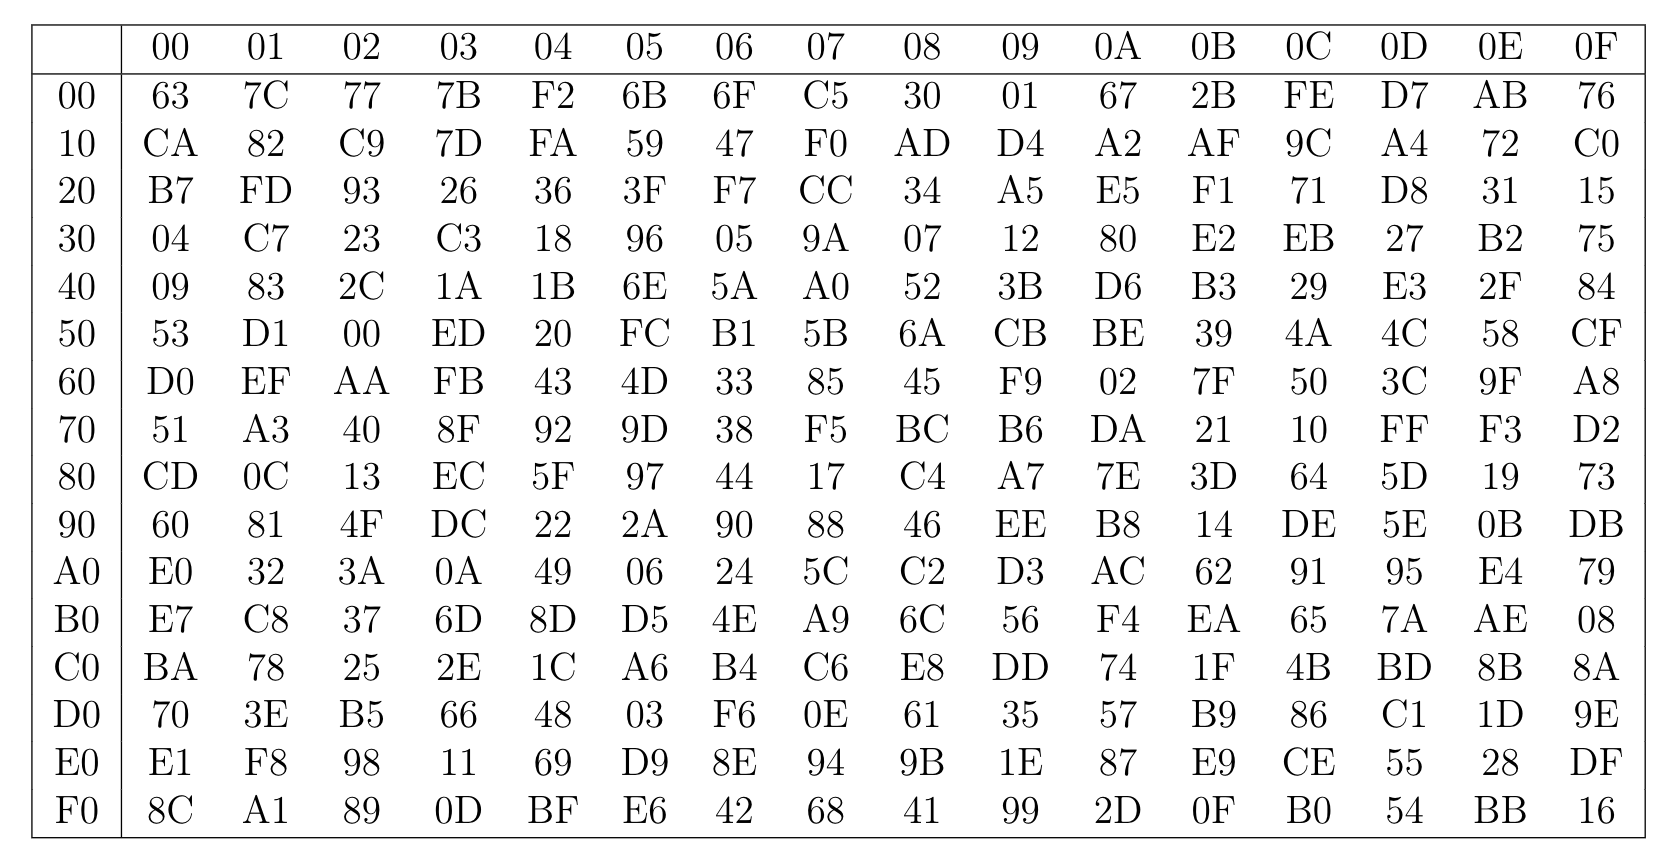
\includegraphics[width=14cm]{./fig/aes_sbox.png}
\end{frame}

% --- NEW SLIDE: AES Pseudocode (Package-Free Version) ---
\begin{frame}{Procedure: \texttt{AES\_Encrypt($\pp, \kk$)}}
    \vspace{-0.8cm}
        \small
        \textbf{Input:} 16-byte array $\pp$, Master-Key $\kk$\\[0.4em]

        $State \gets \pp$ \hfill \textcolor{gray}{\textit{// Initialize $4 \times 4$ byte state matrix}} \\
        $W \gets \text{KeyExpansion}(K)$ \hfill \textcolor{gray}{\textit{// Generate round keys}} \\[0.4em]

        \text{AddRoundKey}($State, W[0]$) \hfill \textcolor{gray}{\textit{// Initial AddRoundKey}} \\[0.1em]

        \textbf{for} $round \gets 1$ \textbf{to} $N_r - 1$ \textbf{do} \hfill \textcolor{gray}{\textit{// $N_r = 10, 12, \text{ or } 14$}} \\
        \hspace*{2em} \text{SubBytes}($State$) \\
        \hspace*{2em} \text{ShiftRows}($State$) \\
        \hspace*{2em} \text{MixColumns}($State$) \\
        \hspace*{2em} \text{AddRoundKey}($State, W[round]$) \\ [0.1em]

        \text{SubBytes}($State$) \hfill \textcolor{gray}{\textit{// Final round (No MixColumns)}} \\
        \text{ShiftRows}($State$) \\
        \text{AddRoundKey}($State, W[N_r]$) \\[0.4em]

        \textbf{return} $out$ ($\cc$)
\end{frame}
% --- NEW SLIDE: AES Decryption Pseudocode ---
\begin{frame}{Procedure: \texttt{AES\_Decrypt($\cc, \kk$)}}
    \vspace{-0.8cm}
        \small
        \textbf{Input:} 16-byte array $\cc$, Master-Key $\kk$\\[0.4em]

        $State \gets \cc$ \hfill \textcolor{gray}{\textit{// Initialize state with the ciphertext}} \\
        $W \gets \text{KeyExpansion}(K)$ \hfill \textcolor{gray}{\textit{// Generate same round keys as encryption}} \\[0.4em]

        \text{AddRoundKey}($State, W[N_r]$) \hfill \textcolor{gray}{\textit{// Use the last round key first}} \\[0.1em]

        \textbf{for} $round \gets N_r - 1$ \textbf{down to} $1$ \textbf{do} \hfill \textcolor{gray}{\textit{// Iterate backwards}} \\
        \hspace*{2em} \red{\text{InvShiftRows}($State$)} \\
        \hspace*{2em} \text{InvSubBytes}($State$) \\
        \hspace*{2em} \text{AddRoundKey}($State, W[round]$) \\
        \hspace*{2em} \text{InvMixColumns}($State$) \\ [0.1em]

        \text{InvShiftRows}($State$) \hfill \textcolor{gray}{\textit{// Final round (No InvMixColumns)}} \\
        \text{InvSubBytes}($State$) \\
        \text{AddRoundKey}($State, W[0]$) \hfill \textcolor{gray}{\textit{// Use the first round key last}}\\[0.4em]

        \textbf{return} $State$ ($\pp$)
\end{frame}

\begin{frame}{Comparison of Encryption and Decryption}
\begin{center}
    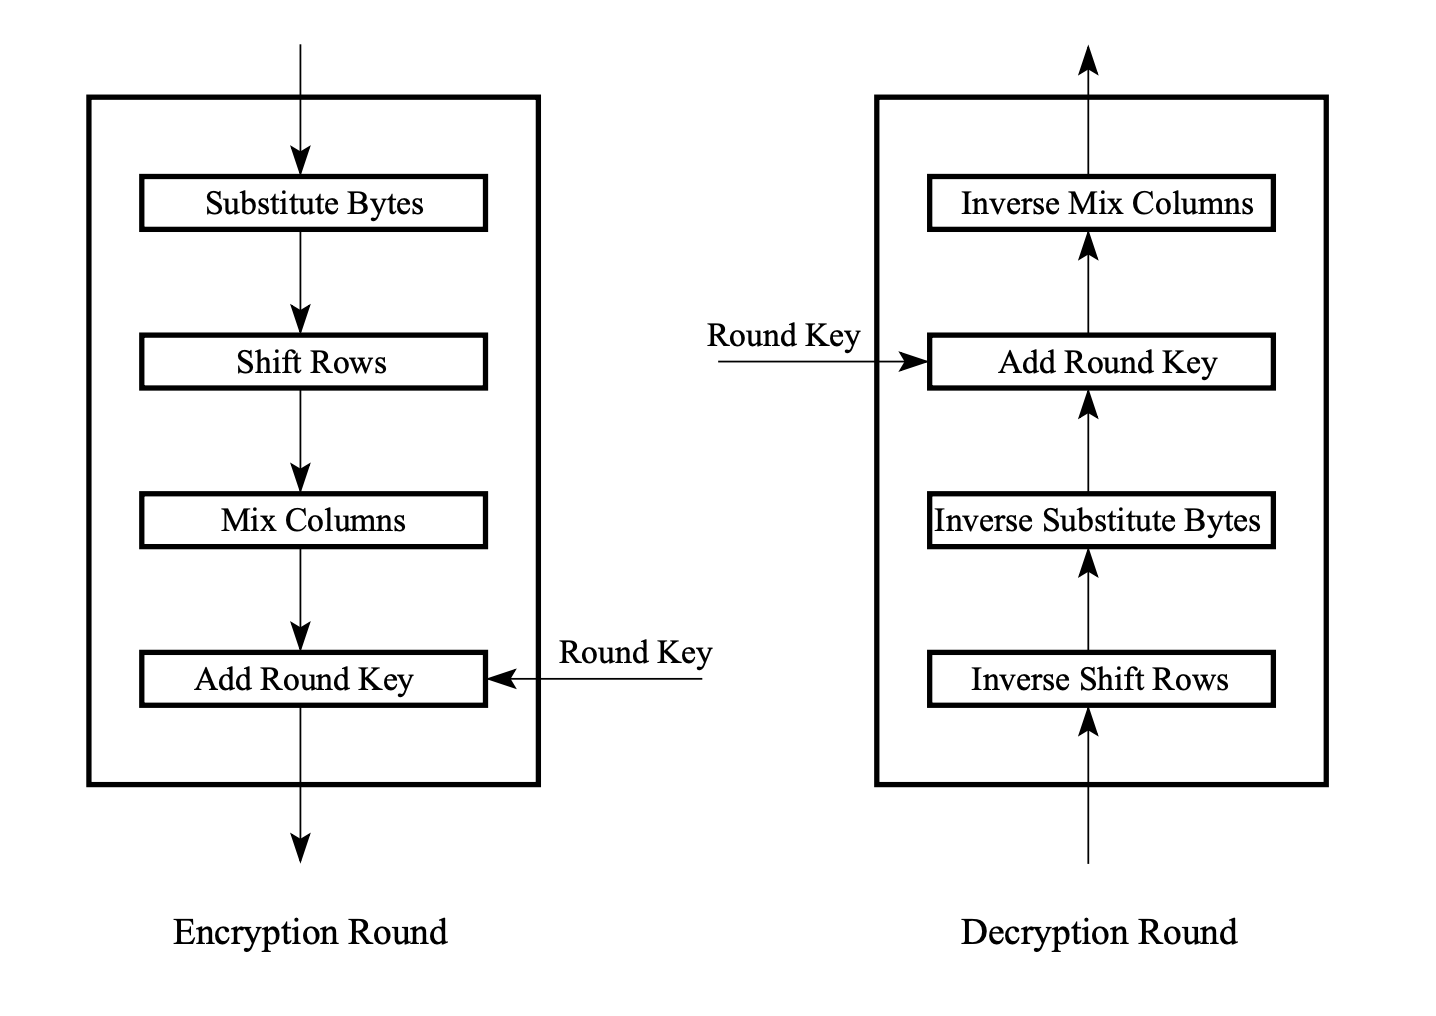
\includegraphics[width=0.8\textwidth]{./fig/enc_dec.png}
\end{center}
\end{frame}
% --- SLIDE 6 through 19 (Animation) ---
\begin{frame}{\tx{AES} Key Schedule Algorithm}
    Master-Key size = $32 \cdot Nk$-bit key (e.g., $Nk = 4$ for \tx{AES-128})
    \pause
    \begin{itemize}
        \item Initialize: $W[0, \dots, Nk-1] = \kk[0, \dots, Nk-1]$.
        \pause
        \item For $i = Nk, \dots, 4 \cdot (7 + Nk) - 1$ do \\[0.4em]
        \pause
        \begin{itemize}
            \item If $i \equiv 0 \pmod{Nk}$ then \\
            $W[i] = W[i-Nk] \oplus {} \text{SB}(W[i-1] \lll 8) \oplus RCON[i/Nk]$,
            \vspace{0.2em}
            \item Else if $Nk \equiv 8$ and $i \equiv 4 \pmod 8$ then \\
            $W[i] = W[i-8] \oplus \text{SB}(W[i-1])$,
            \vspace{0.2em}
            \item Otherwise \\
            $W[i] = W[i-1] \oplus W[i-Nk]$,
        \end{itemize}
        \pause
        \vspace{0.4em}
        \item The first subkey is $W[0, 1, 2, 3]$, the second is $W[4, 5, 6, 7]$, etc.
    \end{itemize}
\end{frame}

\begin{frame}{\tx{AES} Key Schedule}
\begin{columns}[t]

\begin{column}{0.2\textwidth}
\begin{center}
\begin{tikzpicture}[scale=0.5, transform shape, font=\sffamily]
\begin{scope}[xshift=0cm]
    \draw (0,0) rectangle (4,4);
    \draw (0,1) -- +(4,0);
    \draw (0,2) -- +(4,0);
    \draw (0,3) -- +(4,0);
    \draw (1,0) -- +(0,4);
    \draw (2,0) -- +(0,4);
    \draw (3,0) -- +(0,4);
  \end{scope}

  \begin{scope}[yshift=-9cm]
    \draw (0,0) rectangle (4,4);
    \draw (0,1) -- +(4,0);
    \draw (0,2) -- +(4,0);
    \draw (0,3) -- +(4,0);
    \draw (1,0) -- +(0,4);
    \draw (2,0) -- +(0,4);
    \draw (3,0) -- +(0,4);
  \end{scope}

  \draw[->] (0.5,0) -- ++(0,-1+0.25);
  \draw[] (0.5,-1) circle (0.25);
  \draw[] (0.25,-1) -- ++(0.5,0);  
  \draw[->] (3.5,-1) -- ++(-3+0.25,0);
  \draw[fill=white] (2.5+0.2,-1-0.25) rectangle node{\large\texttt{<<}} ++(1-0.4,0.5);
  \draw[fill=white] (1.5+0.2,-1-0.25) rectangle node{\textsf{S}} ++(1-0.4,0.5);
  \draw[->] (0.5,-1+0.25) -- ++(0,-4.5+0.25);

  \draw[->] (1.5,0) -- ++(0,-2+0.25);
  \draw[->] (1.5,-2+0.25) -- ++(0,-3.25);
  \draw[->] (0.5, -2) -- ++(1-0.25,0);
  \draw[]   (1.5,-2) circle (0.25);
  \draw[]   (1.25,-2) -- ++(0.5,0);  
  
  \draw[->] (2.5,0) -- ++(0,-3+0.25);
  \draw[->] (2.5,-3+0.25) -- ++(0,-2.25);
  \draw[->] (1.5, -3) -- ++(1-0.25,0);
  \draw[]   (2.5,-3) circle (0.25);
  \draw[]   (2.25,-3) -- ++(0.5,0);  

  \draw[->] (3.5,0) -- ++(0,-4+0.25);
  \draw[->] (3.5,-4+0.25) -- ++(0,-1.25);
  \draw[->] (2.5, -4) -- ++(1-0.25,0);
  \draw[]   (3.5,-4) circle (0.25);
  \draw[]   (3.25,-4) -- ++(0.5,0);  

\end{tikzpicture}
\end{center}
\end{column}

\begin{column}{0.3\textwidth}
\begin{center}
\begin{tikzpicture}[scale=0.42, transform shape, font=\sffamily]
    \begin{scope}[xshift=0cm]
    \draw (0,0) rectangle (6,4);
    \draw (0,1) -- +(6,0);
    \draw (0,2) -- +(6,0);
    \draw (0,3) -- +(6,0);
    \draw (1,0) -- +(0,4);
    \draw (2,0) -- +(0,4);
    \draw (3,0) -- +(0,4);
    \draw (4,0) -- +(0,4);
    \draw (5,0) -- +(0,4);
  \end{scope}

  \begin{scope}[yshift=-11cm]
    \draw (0,0) rectangle (6,4);
    \draw (0,1) -- +(6,0);
    \draw (0,2) -- +(6,0);
    \draw (0,3) -- +(6,0);
    \draw (1,0) -- +(0,4);
    \draw (2,0) -- +(0,4);
    \draw (3,0) -- +(0,4);
    \draw (4,0) -- +(0,4);
    \draw (5,0) -- +(0,4);
  \end{scope}

  \draw[->] (0.5,0) -- ++(0,-1+0.25);
  \draw[] (0.5,-1) circle (0.25);
  \draw[] (0.25,-1) -- ++(0.5,0);
  \draw[->] (5.5,-1) -- ++(-5+0.25,0);
  \draw[fill=white] (4.5+0.2,-1-0.25) rectangle node{\large\texttt{<<}} ++(1-0.4,0.5);
  \draw[fill=white] (3.5+0.2,-1-0.25) rectangle node{\large\textsf{S}} ++(1-0.4,0.5);
  \draw[->] (0.5,-1+0.25) -- ++(0,-6.5+0.25);

  \draw[->] (1.5,0) -- ++(0,-2+0.25);
  \draw[->] (1.5,-2+0.25) -- ++(0,-5.25);
  \draw[->] (0.5, -2) -- ++(1-0.25,0);
  \draw[]   (1.5,-2) circle (0.25);
  \draw[]   (1.25,-2) -- ++(0.5,0);

  \draw[->] (2.5,0) -- ++(0,-3+0.25);
  \draw[->] (2.5,-3+0.25) -- ++(0,-4.25);
  \draw[->] (1.5, -3) -- ++(1-0.25,0);
  \draw[]   (2.5,-3) circle (0.25);
  \draw[]   (2.25,-3) -- ++(0.5,0);

  \draw[->] (3.5,0) -- ++(0,-4+0.25);
  \draw[->] (3.5,-4+0.25) -- ++(0,-3.25);
  \draw[->] (2.5, -4) -- ++(1-0.25,0);
  \draw[]   (3.5,-4) circle (0.25);
  \draw[]   (3.25,-4) -- ++(0.5,0);

  \draw[->] (4.5,0) -- ++(0,-5+0.25);
  \draw[->] (4.5,-5+0.25) -- ++(0,-2.25);
  \draw[->] (3.5, -5) -- ++(1-0.25,0);
  \draw[]   (4.5,-5) circle (0.25);
  \draw[]   (4.25,-5) -- ++(0.5,0);

  \draw[->] (5.5,0) -- ++(0,-6+0.25);
  \draw[->] (5.5,-6+0.25) -- ++(0,-1.25);
  \draw[->] (4.5, -6) -- ++(1-0.25,0);
  \draw[]   (5.5,-6) circle (0.25);
  \draw[]   (5.25,-6) -- ++(0.5,0);
\end{tikzpicture}
\end{center}
\end{column}

\begin{column}{0.4\textwidth}
\begin{center}
\begin{tikzpicture}[scale=0.35, transform shape, font=\sffamily]
    \begin{scope}[xshift=0cm]
    \draw (0,0) rectangle (8,4);
    \draw (0,1) -- +(8,0);
    \draw (0,2) -- +(8,0);
    \draw (0,3) -- +(8,0);
    \draw (1,0) -- +(0,4);
    \draw (2,0) -- +(0,4);
    \draw (3,0) -- +(0,4);
    \draw (4,0) -- +(0,4);
    \draw (5,0) -- +(0,4);
    \draw (6,0) -- +(0,4);
    \draw (7,0) -- +(0,4);
  \end{scope}

  \begin{scope}[yshift=-14cm]
    \draw (0,0) rectangle (8,4);
    \draw (0,1) -- +(8,0);
    \draw (0,2) -- +(8,0);
    \draw (0,3) -- +(8,0);
    \draw (1,0) -- +(0,4);
    \draw (2,0) -- +(0,4);
    \draw (3,0) -- +(0,4);
    \draw (4,0) -- +(0,4);
    \draw (5,0) -- +(0,4);
    \draw (6,0) -- +(0,4);
    \draw (7,0) -- +(0,4);
  \end{scope}

  \draw[->] (0.5,0) -- ++(0,-1+0.25);
  \draw[] (0.5,-1) circle (0.25);
  \draw[] (0.25,-1) -- ++(0.5,0);
  \draw[->] (7.5,-1) -- ++(-7+0.25,0);
  \draw[fill=white] (6.5+0.2,-1-0.25) rectangle node{\large\texttt{<<}} ++(1-0.4,0.5);
  \draw[fill=white] (5.5+0.2,-1-0.25) rectangle node{\large\textsf{S}} ++(1-0.4,0.5);
  \draw[->] (0.5,-1+0.25) -- ++(0,-9.5+0.25);

  \draw[->] (1.5,0) -- ++(0,-2+0.25);
  \draw[->] (1.5,-2+0.25) -- ++(0,-8.25);
  \draw[->] (0.5, -2) -- ++(1-0.25,0);
  \draw[]   (1.5,-2) circle (0.25);
  \draw[]   (1.25,-2) -- ++(0.5,0);

  \draw[->] (2.5,0) -- ++(0,-3+0.25);
  \draw[->] (2.5,-3+0.25) -- ++(0,-7.25);
  \draw[->] (1.5, -3) -- ++(1-0.25,0);
  \draw[]   (2.5,-3) circle (0.25);
  \draw[]   (2.25,-3) -- ++(0.5,0);

  \draw[->] (3.5,0) -- ++(0,-4+0.25);
  \draw[->] (3.5,-4+0.25) -- ++(0,-6.25);
  \draw[->] (2.5, -4) -- ++(1-0.25,0);
  \draw[]   (3.5,-4) circle (0.25);
  \draw[]   (3.25,-4) -- ++(0.5,0);

  \draw[->] (4.5,0) -- ++(0,-6+0.25);
  \draw[->] (4.5,-6+0.25) -- ++(0,-4.25);
  \draw[->] (3+0.5, -5+0.5) -- ++(0.5,0) -- ++(0,-1.5) -- ++(0.5-0.25,0);
  \draw[fill=white] (3.5+0.2,-5.5) rectangle node{\large\textsf{S}} ++(1-0.4,0.5);
  \draw[]   (4.5,-6) circle (0.25);
  \draw[]   (4.25,-6) -- ++(0.5,0);

  \draw[->] (5.5,0) -- ++(0,-7+0.25);
  \draw[->] (5.5,-7+0.25) -- ++(0,-3.25);
  \draw[->] (4.5, -7) -- ++(1-0.25,0);
  \draw[]   (5.5,-7) circle (0.25);
  \draw[]   (5.25,-7) -- ++(0.5,0);

  \draw[->] (6.5,0) -- ++(0,-8+0.25);
  \draw[->] (6.5,-8+0.25) -- ++(0,-2.25);
  \draw[->] (5.5, -8) -- ++(1-0.25,0);
  \draw[]   (6.5,-8) circle (0.25);
  \draw[]   (6.25,-8) -- ++(0.5,0);

  \draw[->] (7.5,0) -- ++(0,-9+0.25);
  \draw[->] (7.5,-9+0.25) -- ++(0,-1.25);
  \draw[->] (6.5, -9) -- ++(1-0.25,0);
  \draw[]   (7.5,-9) circle (0.25);
  \draw[]   (7.25,-9) -- ++(0.5,0);

\end{tikzpicture}
\end{center}
\end{column}


\end{columns}
\end{frame}


\section{The Feistel Structure and \tx{DES}}
% --- SLIDE 2: The Feistel Structure (Visual + Math) ---
\begin{frame}
    \frametitle{The Feistel Structure}
    \begin{columns}[c] % Vertically centered columns
        \begin{column}{0.3\textwidth}
            \feisteldiagram % Use our new command
        \end{column}

        \begin{column}{0.6\textwidth}
            \begin{block}{Encryption Round}
                \begin{align*}
                    L_{i+1} &= R_i \\
                    R_{i+1} &= L_i \oplus F(K_{i}, R_i)
                \end{align*}
            \end{block}
        \end{column}
    \end{columns}
\end{frame}

% --- SLIDE 3: Case 1 ---
\begin{frame}[fragile]
    \frametitle{Exploring Weak Functions}
    \begin{columns}[T] % Top-aligned columns
        \begin{column}{0.5\textwidth}
            \feisteldiagram % The diagram remains
        \end{column}

        \begin{column}{0.5\textwidth}
            \begin{block}{Case 1: The Zero Function}
                What if $F(K, x) = 0 \forall x$?
            \end{block}

            \pause

            \uncover<2->{$
            \begin{aligned}[t]
                L_1 &= R_0 \\ R_1 &= L_0 \oplus 0 = L_0 \\
            \end{aligned}
            $}

            \uncover<3->{$
            \begin{aligned}[t]
                L_2 &= L_0  \\ R_2 &= R_0 \\
            \end{aligned}
            $}

            \uncover<4->{
            \begin{alertblock}{Result}
                After an even number of rounds, you get the input back. \red{No security!}
            \end{alertblock}}
        \end{column}
    \end{columns}
\end{frame}

% --- SLIDE 4: Case 2 ---
\begin{frame}[fragile]
    \frametitle{Exploring Weak Functions}
    \begin{columns}[T]
        \begin{column}{0.5\textwidth}
            \feisteldiagram % The diagram remains
        \end{column}

        \begin{column}{0.5\textwidth}
            \begin{block}{Case 2: The Identity Function}
                What if $F(K, x) = x, \forall x$?
            \end{block}

            \uncover<2->{$
            \begin{aligned}[t]
                L_1 &= R_0 \\ R_1 &= L_0 \oplus R_0 \\
            \end{aligned}
            $}

            \uncover<3->{$
            \begin{aligned}[t]
                L_2 &= L_0 \oplus R_0 \\ R_2 &= R_0 \oplus (L_0 \oplus R_0) = L_0 \\
            \end{aligned}
            $}

            \uncover<4->{$
            \begin{aligned}[t]
                L_3 &= L_0 \\ R_3 &= (L_0 \oplus R_0) \oplus L_0 = R_0
            \end{aligned}
            $}

            \uncover<4->{
            \begin{alertblock}{Result}
                The input $(L_0, R_0)$ is restored after just 3 rounds. \red{No security!}
            \end{alertblock}}
        \end{column}
    \end{columns}
\end{frame}

% --- SLIDE 5: Case 3 ---
\begin{frame}[fragile]
    \frametitle{Exploring Weak Functions}
    \begin{columns}[T]
        \begin{column}{0.5\textwidth}
            \feisteldiagram % The diagram remains
        \end{column}

        \begin{column}{0.5\textwidth}
            \begin{block}{Case 3: Simple XOR with Key}
                What if $F(K, x) = K \oplus x \forall x$?
            \end{block}

            \pause
            \uncover<2->{$
            \begin{aligned}[t]
                L_1 &= R_0 \\
                R_1 &= L_0 \oplus R_0 \oplus K_1 \\
            \end{aligned}
            $}
            \uncover<3->{$
            \begin{aligned}[t]
                L_2 &= L_0 \oplus R_0 \oplus K_1 \\
                R_2 &= R_0 \oplus (L_0 \oplus L_2) \oplus K_2 \\
                   &= L_0 \oplus K_1 \oplus K_2
            \end{aligned}
            $}

            \pause

            \uncover<3->{
            \begin{alertblock}{Result}
                The output is just a linear function of the input and keys. Broken with basic algebra. \red{No security!}
            \end{alertblock}}
        \end{column}
    \end{columns}
\end{frame}

% --- SLIDE 6: Conclusion (No diagram needed here) ---
\begin{frame}
    \frametitle{Conclusion: The Round Function is Everything}

    \begin{block}{Main Lesson}
        A Feistel network is excellent \textbf{structure}, but its \textbf{round function} is everything.
    \end{block}

    \begin{itemize}
        \item<2-> Weak or simple $F$ functions lead to ciphers that are trivially broken.
        \item<3-> A strong $F$ function must be \textbf{non-linear}
    \end{itemize}

\end{frame}


\begin{frame}
    \begin{columns}[t]
        \begin{column}{0.50\linewidth}
            \begin{figure}[!h]
                \centering
                
\includegraphics[width=5.7cm]{./img/web.png}
            \end{figure}
        \end{column}
        \begin{column}{0.50\linewidth}
            \begin{center}
                {\huge {\color{red} Thank You} for your attention!} \\ \Large Any questions?
            \end{center}
        \end{column}
    \end{columns}
\end{frame}

\bibliographystyle{alpha}
\bibliography{../bibliography.bib}

\end{document}
